
\chapter{Object Detection}

The object dection model used here is the SSD\footnote{\url{https://arxiv.org/pdf/1512.02325.pdf}}.

The project is the rewrite and simplify the SSD project on github.
Here is the project structure show in Figure \ref{fig:ssd-structure}:
\begin{figure}[!ht]
  \centering
  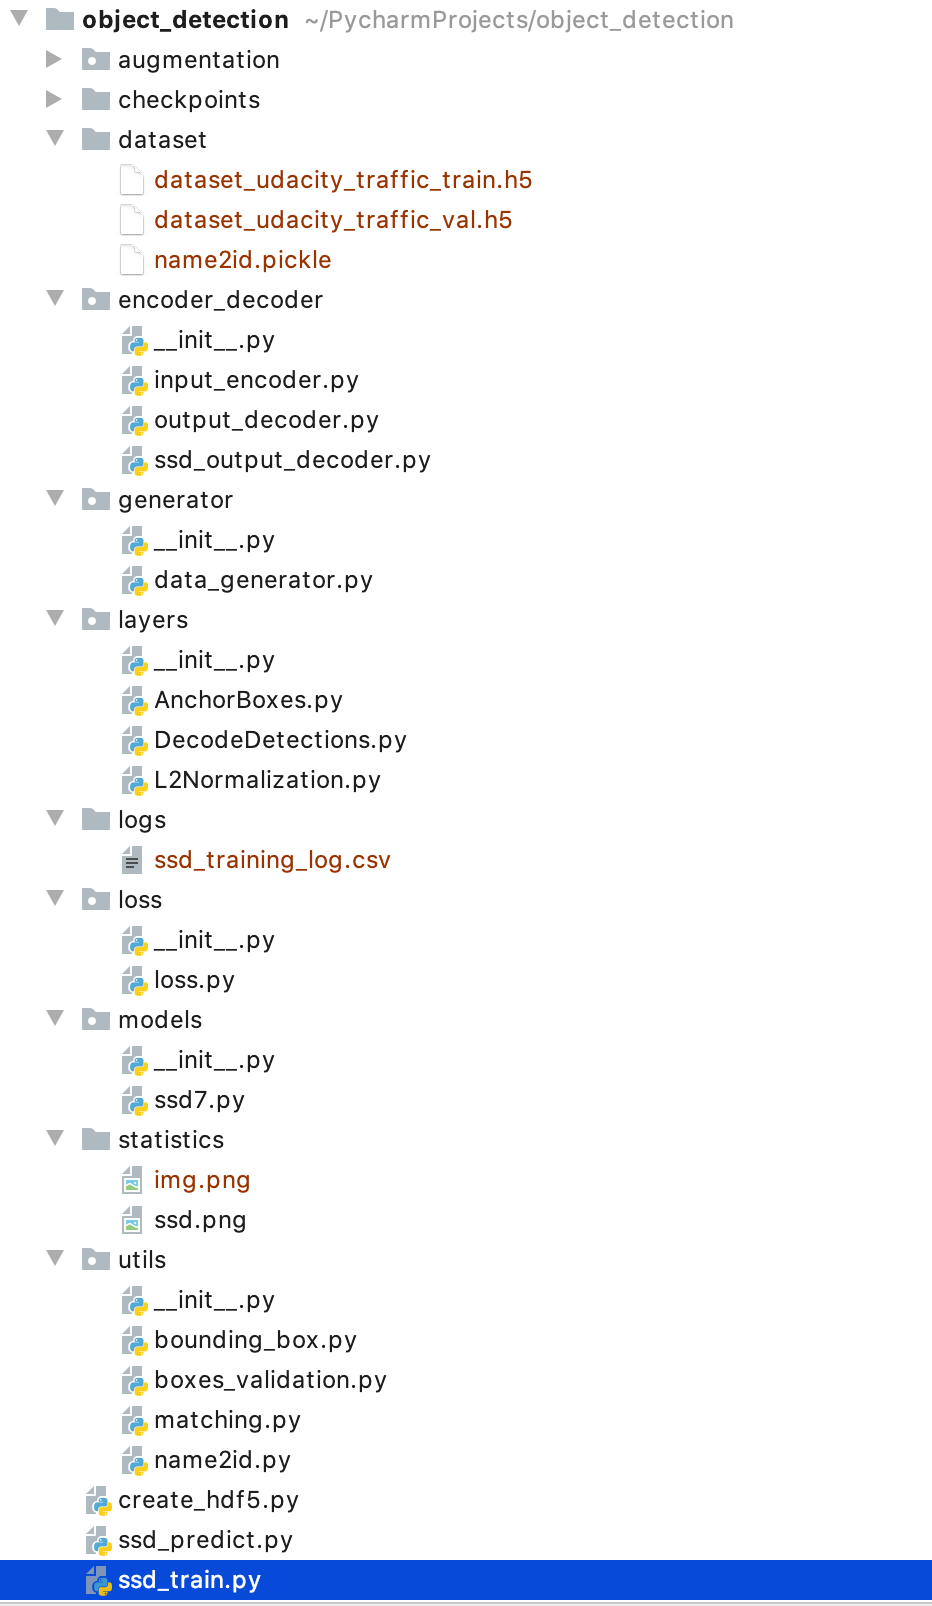
\includegraphics[width=\textwidth]{pics/ssd-structure}
  \caption{SSD structure}
  \label{fig:ssd-structure}
\end{figure}

The project is on the github: \url{https://github.com/mikechyson/object_detection}.


The overview is that:
\begin{enumerate}
\item Use 7 convolution layers to extract feature maps.
\item From layr 4, 5, 6 and 7, extract classes layers, boxes layers and anchors layers.
\item Reshape classes layers, boxes layers and anchors layers.
\item Concatenate classes layers from 4, 5, 6 and 7 convolution layers.
\item Concatenate boxes layers from 4, 5, 6 and 7 convolution layers.
\item Concatenate anchors layers from 4, 5, 6 and 7 convolution layers.
\item Concatenate the contenated classes, boxes and anchors into a whole tensor.
\item Encoder the lables to the same tensor shape with the whole tensor.
\item In training process, compute the loss between the whole tensor and encoded label tensor.
\item In predicting process, decode the whole tensor into classes and boxes tensor.
\end{enumerate}

\section{train.py}


\begin{lstlisting}
import keras.backend as K
from models.ssd7 import build_ssd7
from keras.optimizers import Adam
from loss.loss import SSDLoss
from generator.data_generator import DataGenerator
from augmentation.constant_input_size_chain import DataAugmentationConstantInputSize
from encoder_decoder.input_encoder import SSDInputEncoder
from keras.callbacks import ModelCheckpoint, EarlyStopping, ReduceLROnPlateau, CSVLogger
import math
import matplotlib.pyplot as plt
import numpy as np
from encoder_decoder.output_decoder import decode_detections

########################################################################################################################
# Set the configs
img_height = 300
img_width = 480
img_channels = 3
# Set this to your preference (maybe `None`).
# The current settings transform the input pixel values to the interval `[-1,1]`.
intensity_mean = 127.5
intensity_range = 127.5
n_classes = 5  # Number of positive classes
# An explicit list of anchor box scaling factors.
# If this is passed, it will override `min_scale` and `max_scale`.
scales = [0.08, 0.16, 0.32, 0.64, 0.96]
aspect_ratios = [0.5, 1.0, 2.0]  # The list of aspect ratios for the anchor boxes
two_boxes_for_ar1 = True  # Whether or not you want to generate two anchor boxes for aspect ratio 1
steps = None  # In case you'd like to set the step sizes for the anchor box grids manually; not recommended
offsets = None  # In case you'd like to set the offsets for the anchor box grids manually; not recommended
clip_boxes = False  # Whether or not to clip the anchor boxes to lie entirely within the image boundaries
variances = [1.0, 1.0, 1.0, 1.0]  # The list of variances by which the encoded target coordinates are scaled
normalize_coords = True  # Whether or not the model is supposed to use coordinates relative to the image size
batch_size = 16

########################################################################################################################
# Create the model
K.clear_session()  # Clear previous models from memory.
model = build_ssd7(image_size=(img_height, img_width, img_channels),
                   n_classes=n_classes,
                   mode='training',
                   l2_regularization=0.0005,
                   scales=scales,
                   aspect_ratios_global=aspect_ratios,
                   aspect_ratios_per_layer=None,
                   two_boxes_for_ar1=two_boxes_for_ar1,
                   steps=steps,
                   offsets=offsets,
                   clip_boxes=clip_boxes,
                   variances=variances,
                   normalize_coords=normalize_coords,
                   subtract_mean=intensity_mean,
                   divide_by_stddev=intensity_range)
print(model.summary())

########################################################################################################################
# Compile the model
adam = Adam(lr=0.001, beta_1=0.9, beta_2=0.999, epsilon=1e-08, decay=0.0)
ssd_loss = SSDLoss(neg_pos_ratio=3, alpha=1.0)
model.compile(optimizer=adam, loss=ssd_loss.compute_loss)

########################################################################################################################
# Set up the data generators for the training
train_dataset = DataGenerator(load_images_into_memory=True,
                              hdf5_dataset_path='dataset/dataset_udacity_traffic_train.h5')
val_dataset = DataGenerator(load_images_into_memory=True,
                            hdf5_dataset_path='dataset/dataset_udacity_traffic_val.h5')

# Get the number of samples in the training and validation datasets.
trail_dataset_size = train_dataset.get_dataset_size()
val_dataset_size = val_dataset.get_dataset_size()
print(f'Number of images in the training dataset  : \t{trail_dataset_size:>6}')
print(f'Number of images in the validation dataset: \t{val_dataset_size:>6}')

########################################################################################################################
# Instantiate an encoder that can encode ground truth labels into the format needed by the SSD loss function.
# The encoder constructor needs the spatial dimensions of the model predictor layers to create the anchor boxes.
predictor_sizes = [
    model.get_layer('classes4').output_shape[1:3],
    model.get_layer('classes5').output_shape[1:3],
    model.get_layer('classes6').output_shape[1:3],
    model.get_layer('classes7').output_shape[1:3]
]
print(f'predictor_sizes={predictor_sizes}')

ssd_input_encoder = SSDInputEncoder(img_height=img_height,
                                    img_width=img_width,
                                    n_classes=n_classes,
                                    predictor_sizes=predictor_sizes,
                                    aspect_ratios_global=aspect_ratios,
                                    two_boxes_for_ar1=two_boxes_for_ar1,
                                    steps=steps,
                                    offsets=offsets,
                                    clip_boxes=clip_boxes,
                                    variances=variances,
                                    matching_type='multi',
                                    pos_iou_threshold=0.5,
                                    neg_iou_limit=0.3,
                                    normalize_coords=normalize_coords)

########################################################################################################################
# Create the generator handles that will be passed to Keras' `fit_generator()` function.
train_generator = train_dataset.generate(batch_size=batch_size,
                                         shuffle=True,
                                         transformations=[],
                                         label_encoder=ssd_input_encoder,
                                         returns={'processed_images', 'encoded_labels'},
                                         keep_images_without_gt=False)
val_generator = val_dataset.generate(batch_size=batch_size,
                                     shuffle=False,
                                     transformations=[],
                                     label_encoder=ssd_input_encoder,
                                     returns={'processed_images', 'encoded_labels'},
                                     keep_images_without_gt=False)

########################################################################################################################
# Define model callbacks.
model_checkpoint = ModelCheckpoint(
    filepath='checkpoints/ssd7_epoch-{epoch:02d}_loss-{loss:.4f}_val_loss-{val_loss:.4f}.h5',
    monitor='val_loss',
    verbose=1,
    save_best_only=True,
    save_weights_only=False,
    mode='auto',
    period=1)
csv_logger = CSVLogger(filename='logs/ssd_training_log.csv',
                       separator=',',
                       append=True)
early_stopping = EarlyStopping(monitor='val_loss',
                               min_delta=0.0,
                               patience=10,
                               verbose=1)
reduce_learning_rate = ReduceLROnPlateau(monitor='val_loss',
                                         factor=0.2,
                                         patience=8,
                                         verbose=1,
                                         epsilon=0.001,
                                         cooldown=0,
                                         min_lr=0.00001)
callbacks = [model_checkpoint, csv_logger, early_stopping, reduce_learning_rate]

########################################################################################################################
# Set the epochs and train.
initial_epoch = 0
final_epoch = 1000
steps_per_epoch = math.ceil(trail_dataset_size / batch_size)

history = model.fit_generator(generator=train_generator,
                              steps_per_epoch=steps_per_epoch,
                              epochs=final_epoch,
                              callbacks=callbacks,
                              validation_data=val_generator,
                              validation_steps=math.ceil(val_dataset_size / batch_size),
                              initial_epoch=initial_epoch,
                              verbose=1)

########################################################################################################################
# Plot the training process.
plt.figure(figsize=(20, 12))
plt.plot(history.history['loss'], label='loss')
plt.plot(history.history['val_loss'], label='val_loss')
plt.legend(loc='upper right', prop={'size': 24})
plt.show()
\end{lstlisting}

The data is stored on netdisk \url{https://pan.baidu.com/s/1cbqyymAHODCiM37DINhwbQ}
The paasword is \verb|snuc|.


The code to convert the data into h5 file is show in \verb|create_hdf5.py|.


Line 148 use the \verb|fit_generator| to fit the data into model and train the model.
This is suitable for large dataset.
For small dataset, you can also you the \verb|fit| method.

\section{ssd\_predict.py}

This is used to predict the object in a image with the trained model.
